\documentclass[aspectratio=169]{beamer}
\usepackage{booktabs}
\usepackage{ulem}
\usepackage{bm}

\usepackage[justification=centering,skip=-5pt,font=footnotesize]{subcaption}
\usepackage{amsmath}
\usepackage{centernot}
\newcommand{\rel}[1]{\xrightarrow{\textrm{#1}}}
\newcommand{\norel}[1]{\centernot{\xrightarrow{\textrm{#1}}}}
%\setbeameroption{show notes}

% Met aspectratio kan je de breedte-hoogteverhouding aanpassen (bijv 1610 = de 
% monitoren op het CBS); 43 is de klassieke verhouding die veel beamers nog
% gebruiken.

\usetheme{cbs}

\title{Development of Educational Segregation Measured using Longitudinal Population Scale Network Data}
\author{{\bf Jan van der Laan \url{<dj.vanderlaan@cbs.nl>}}\\ 
Edwin de Jonge\\Marjolijn Das}
\date{IC${}^\mathrm{2}$S${}^\mathrm{2}$ --- Copenhagen --- July 17--20 2023}

% De institute komt in de voet van de slides naast het nummer; normaal zou hier
% niets moeten staan, maar je kan dit dus misbruiken om iets in de voet van
% de slides te krijgen (bijv datum/naam event)
%\institute{IC${}^\mathrm{2}$S${}^\mathrm{2}$ - July 2020}
%\institute{Methodologiesessie, 8 maart 2021}
\institute{{\tiny IC${}^\mathrm{2}$S${}^\mathrm{2}$ --- Copenhagen --- July 17--20 2023}}

\newcommand{\var}[1]{\mathrm{var}\!\left(#1\right)}
\newcommand{\E}[1]{\mathrm{E}\!\left[#1\right]}

\begin{document}

{
\invert
\usebackgroundtemplate{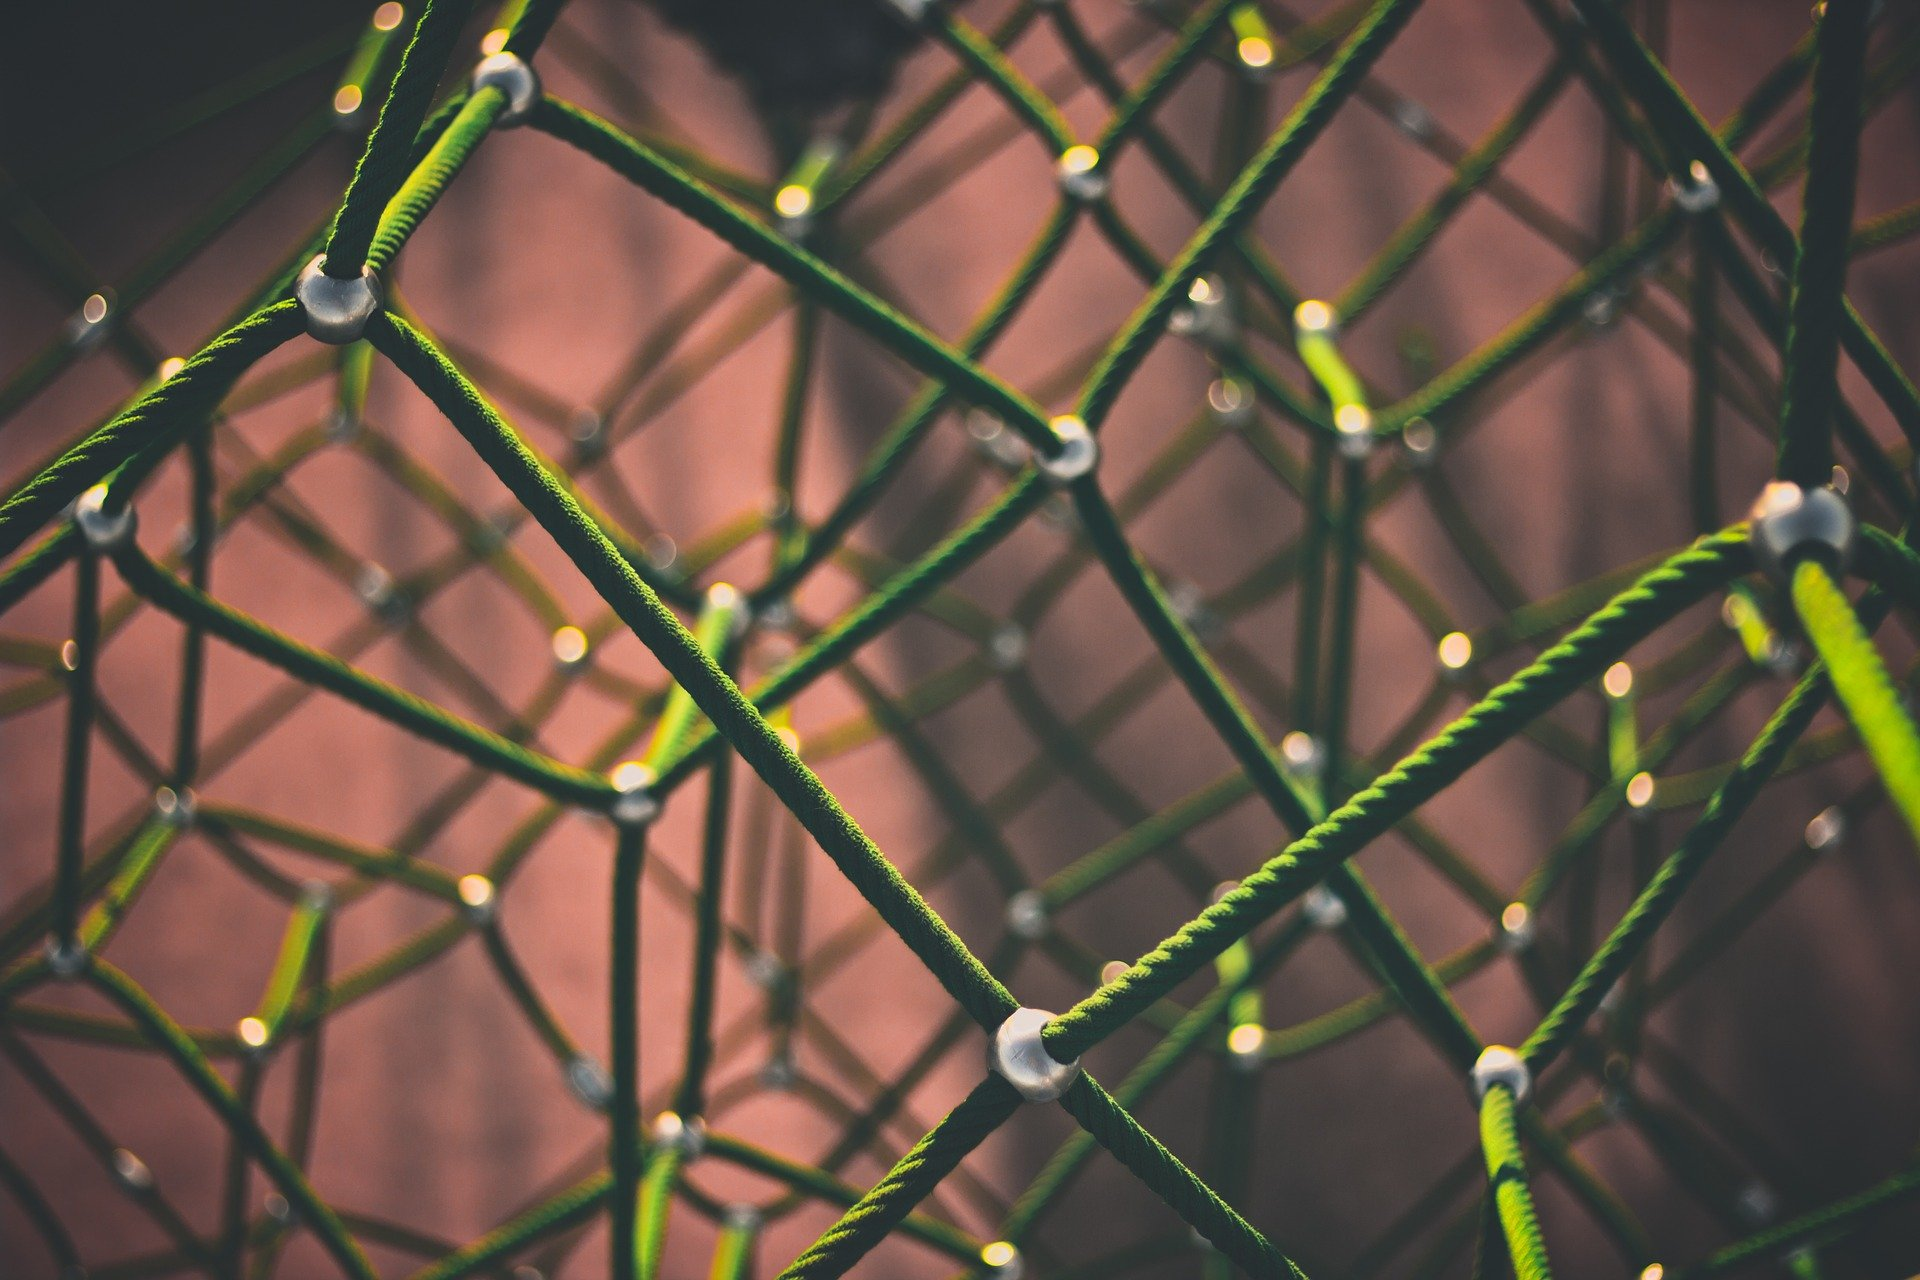
\includegraphics[width=\paperwidth]{figures/bg1.jpg}}
\begin{frame}
  \titlepage
\end{frame}
\revert
}

{
\invert
\begin{frame}{Educational segregation}
  Educational level important predictor of socio-economic success. \\[1em]

  Segregation:
  \begin{itemize}
    \item Polarization and mutual misunderstanding
    \item Reinforce inequality
  \end{itemize}~


  How does the segregation change during a persons life time and how does this change in time?
\end{frame}
\revert
}

\begin{frame}{Person Network of the Netherlands}
  2009--2020 (this study 2013--2020)\\[2em]

  Five layers:
  \begin{itemize}
    \item \textbf{Household}: persons living at the same address
    \item \textbf{Family}: 3rd degree + partner + inlaw + step parents/children
    \item \textbf{Neighbours}: 10 closest households + 20 random persons within 200m
    \item \textbf{Work}: max. 100 closest persons at same company
    \item \textbf{School}: same school, location, study, year.
  \end{itemize}~

  Dense network: 17$\cdot\mathrm{10}^\mathrm{6}$ persons, 2$\cdot\mathrm{10}^\mathrm{9}$ labelled relations
\end{frame}

\begin{frame}{Exposure}
  \textbf{To what extent is a person exposed to the different educational levels?}\\[1em]

  Not only direct contacts relevant, but also indirect contacts.\\[2em]

  Localised random walk / localised page rank ($\alpha$ = 0.4).\\[1em]
  
  \vspace{5em}\scriptsize \it
  Ballester and Vorsatz (2014); Van der Laan \textit{et al.} (2022); \bf De Jonge \textit{et al.} Thursday @ IC2S2
\end{frame}

\begin{frame}{Person transfers some of their values to contacts}
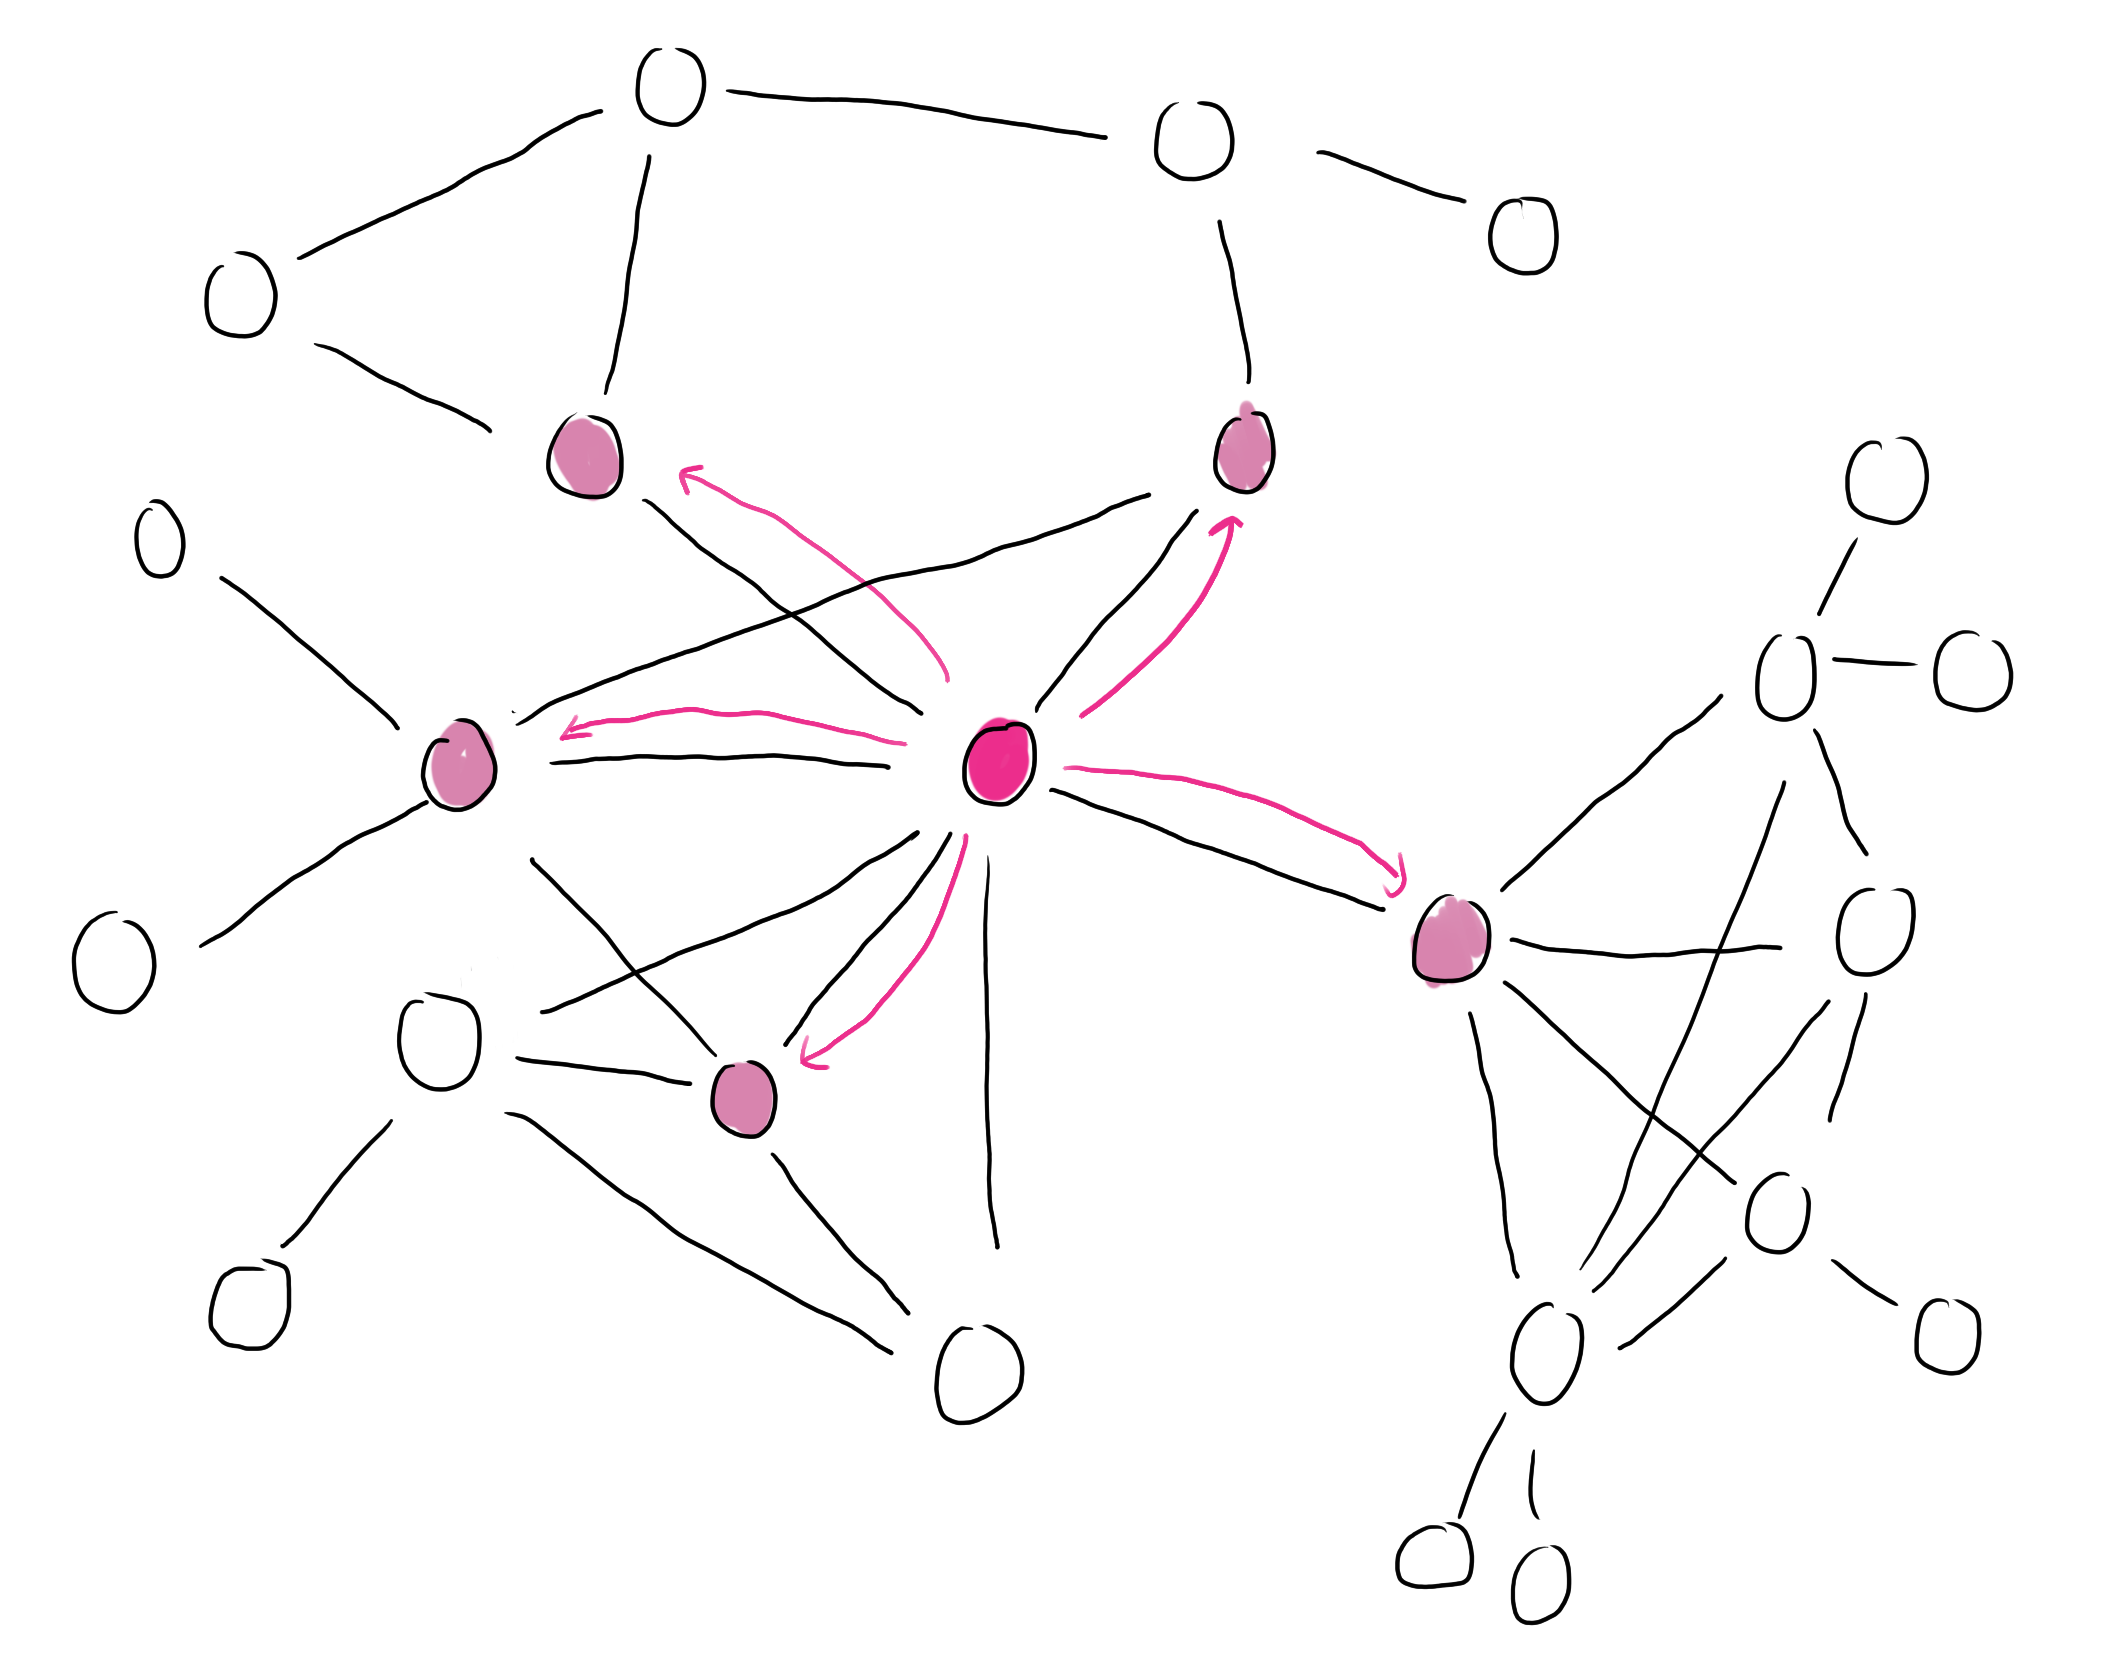
\includegraphics[width=0.52\paperwidth]{figures/random_walk_01.png}
\end{frame}

\begin{frame}{Part of updated values transfered again}
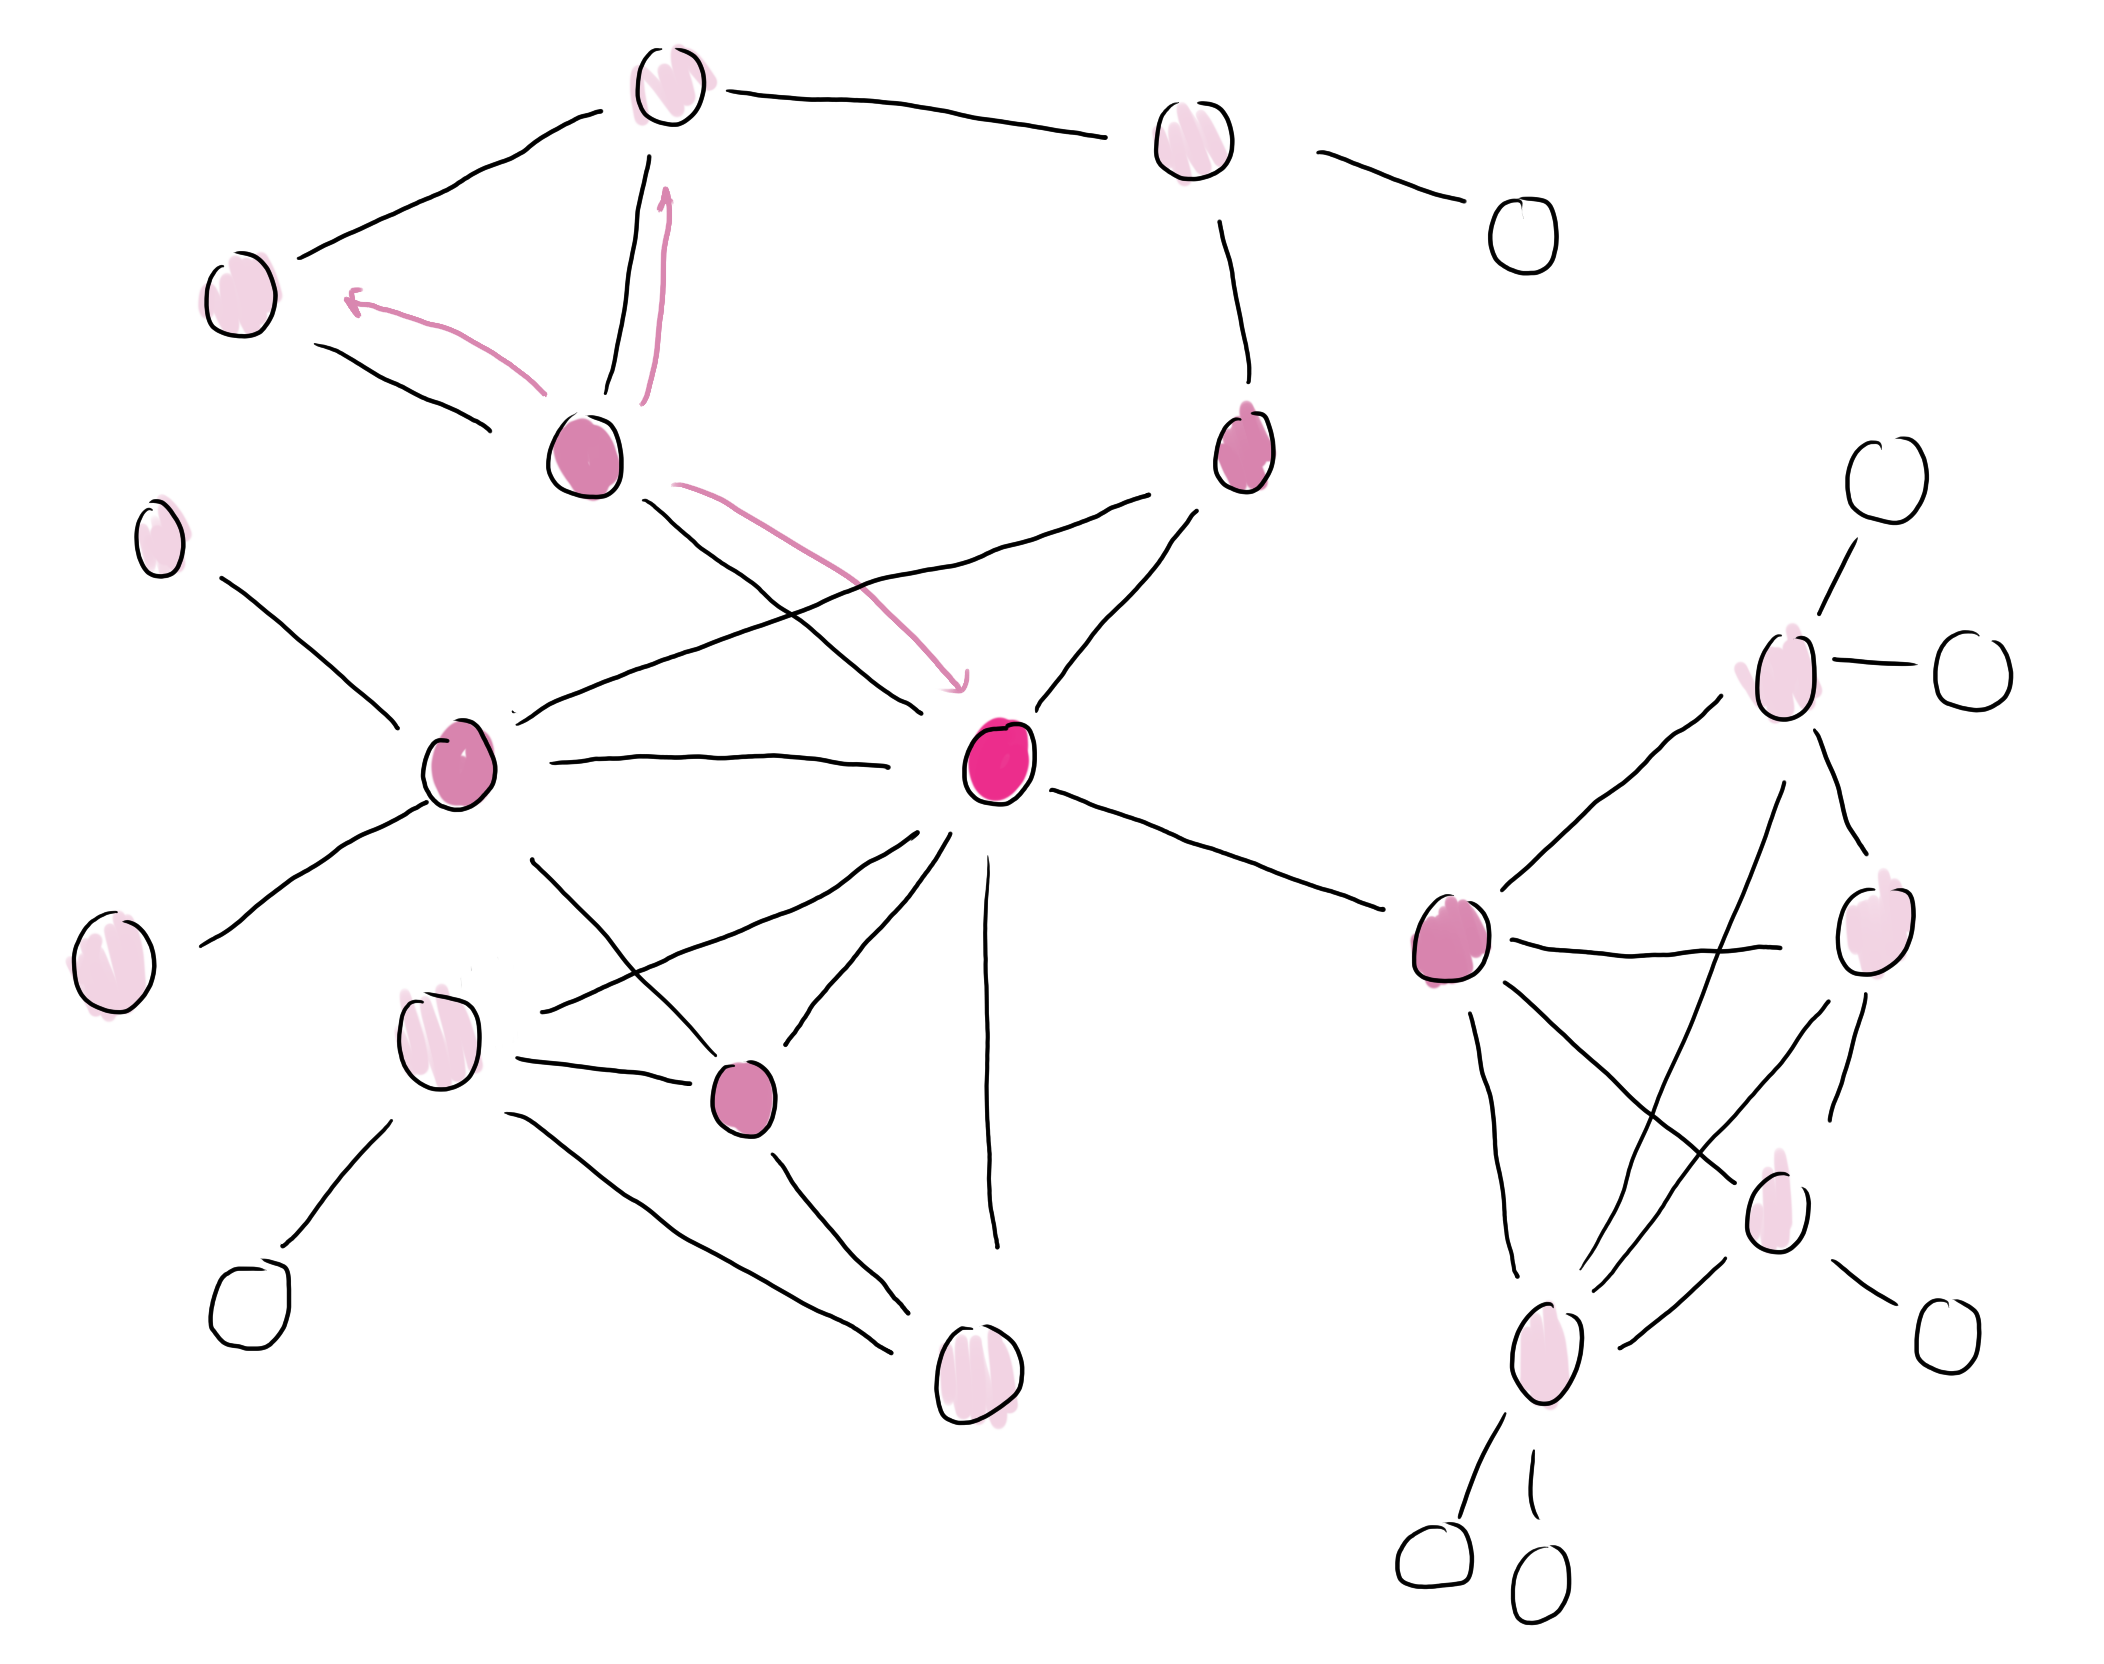
\includegraphics[width=0.52\paperwidth]{figures/random_walk_02.png}
\end{frame}

\begin{frame}{Etc}
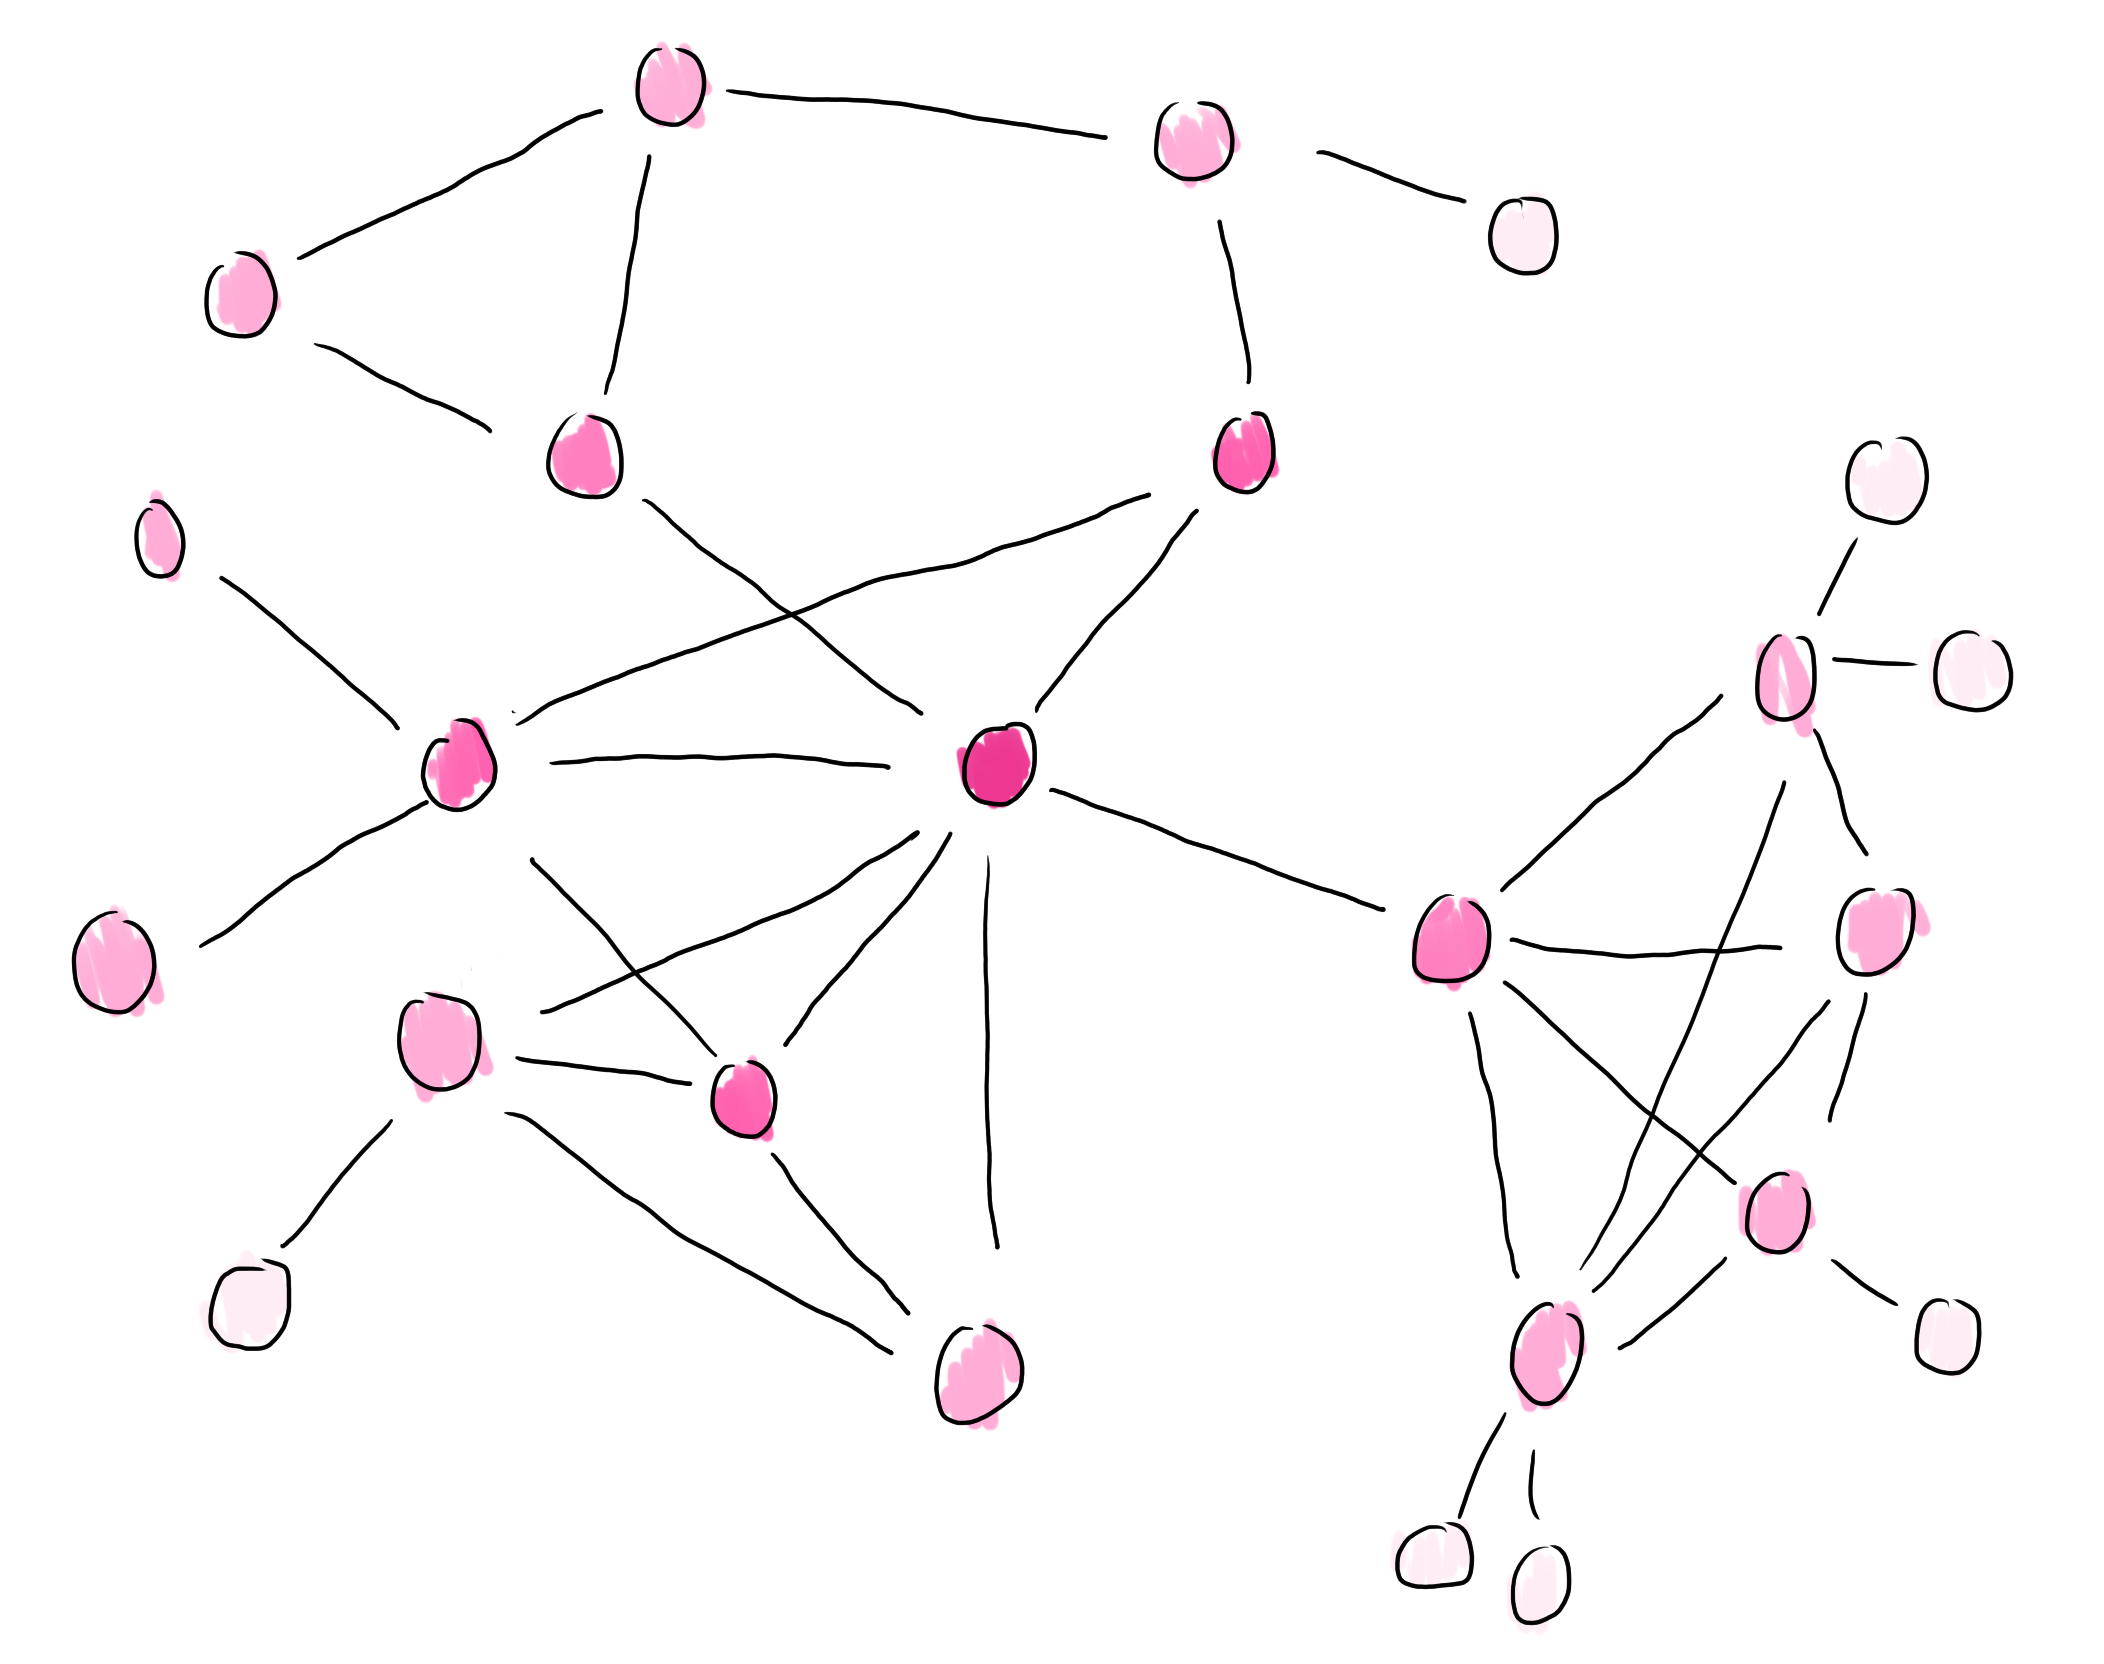
\includegraphics[width=0.52\paperwidth]{figures/random_walk_03.png}
\end{frame}

\begin{frame}{Segregation}
  \textbf{Exposure to own educational level corrected for expected exposure}\\[3em]

  \begin{equation}
    \mathrm{Segregation}_i = \frac{\mathrm{Exposure}_i - \mathrm{ExpectedExposure}_i}{
      1 - \mathrm{ExpectedExposure}_i} \nonumber
  \end{equation}\\[2em]

  Note: measured at individual level\\[0.5em]
  Range 30 km: freedom of choice for forming connections
\end{frame}

\begin{frame}{Segregation as a function of age}
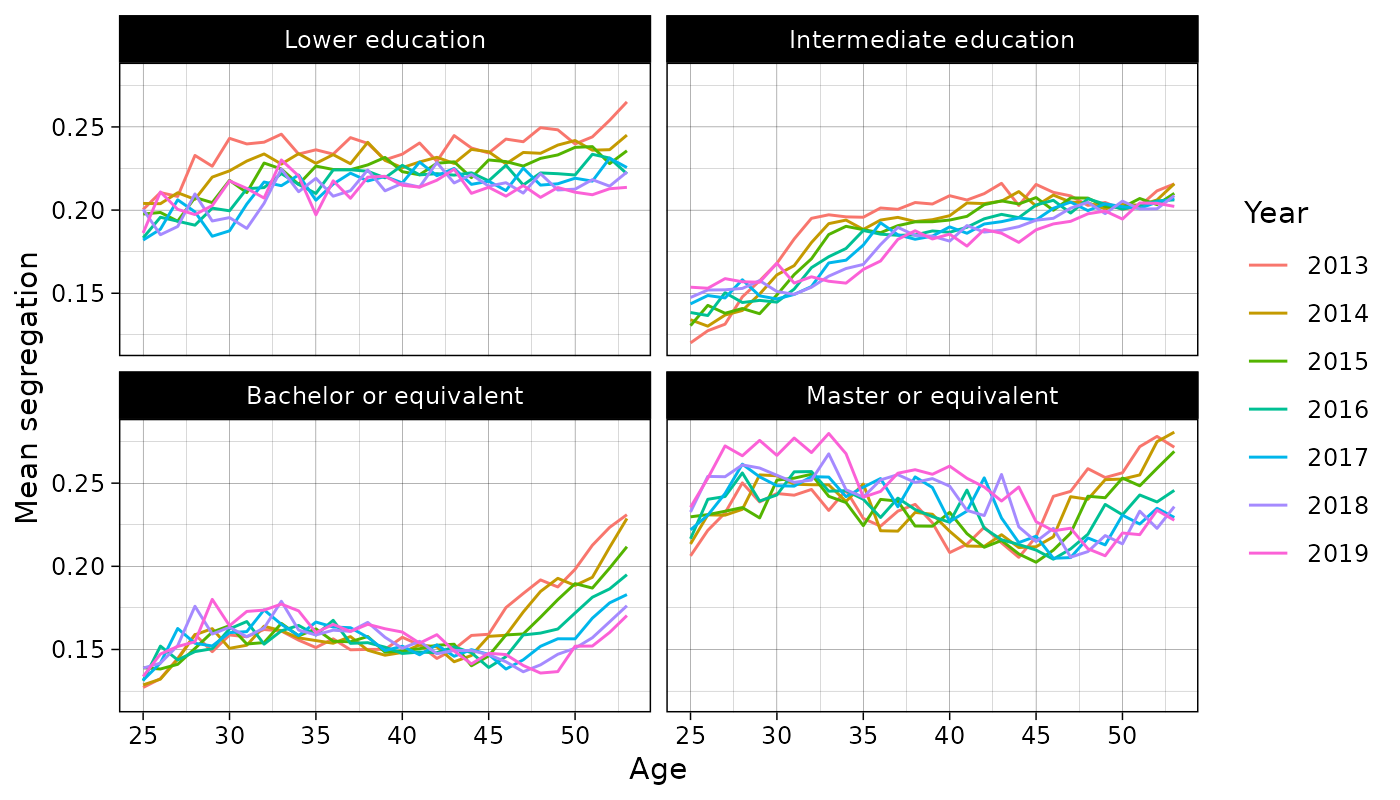
\includegraphics[width=0.79\paperwidth]{figures/segregatie_naar_leeftijd.png}
\end{frame}

\begin{frame}{Average individual year-to-year change}
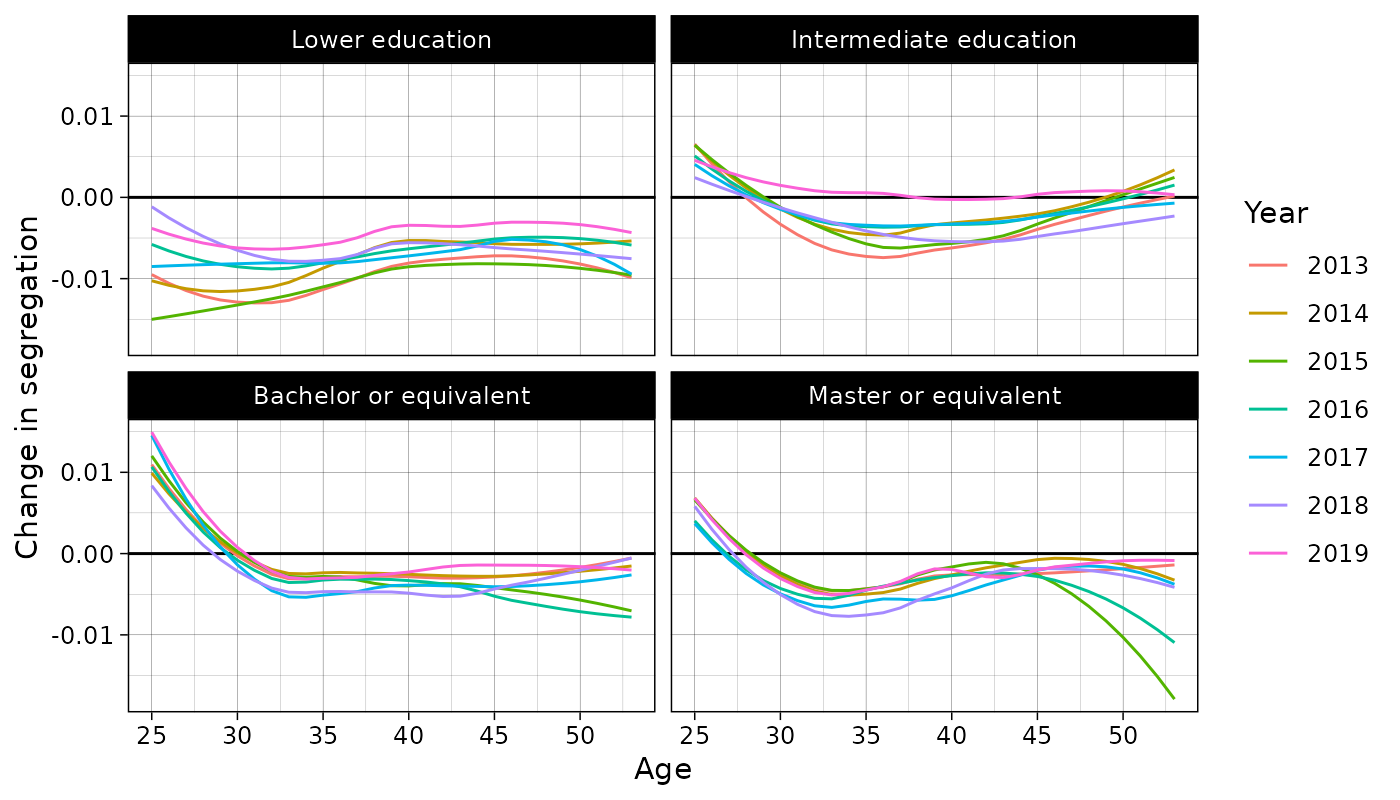
\includegraphics[width=0.79\paperwidth]{figures/segregatie_ontwikkeling_leeftijd.png}
\end{frame}

\begin{frame}{Year-to-year correlation of individual segregation}
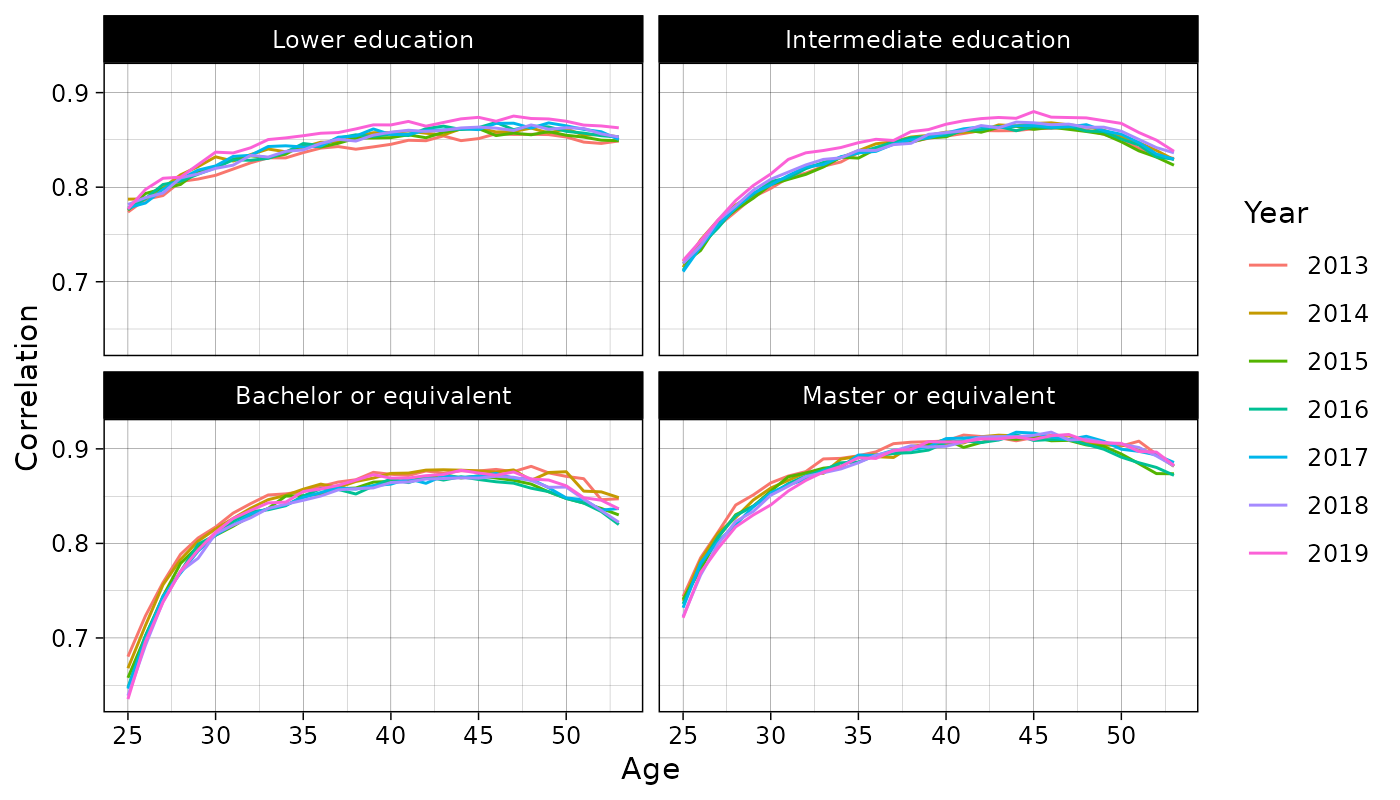
\includegraphics[width=0.79\paperwidth]{figures/correlation.png}
\end{frame}


% =============================================================================
% ==== CONCLUSIE
% =============================================================================

\invert
\begin{frame}{Conclusion}
  Segregation develops until approx. the age of 35.\\[2em]

  After 35 relatively stable (slow decrease).\\[2em]

\end{frame}

\begin{frame}

  \begin{columns}
    \begin{column}{0.67\textwidth}
      {\bf For references and data sources see
      \url{https://github.com/djvanderlaan/papers-ic2s2-2023}\\[2em]
      }

      
  \footnotesize
      C. Ballester and M. Vorsatz, “Random walk-based segregation measures,” Review of Economics and Statistics, vol. 96, pp. 383–401, 2014, doi: 10.1162/REST\_a\_00399.\\[0.5em]
      D. J. van der Laan, E. de Jonge, M. Das, S. Te Riele, and T. Emery, “A whole population network and its application for the social sciences,” European Sociological Review, vol. jcac026, 2022, doi: 10.1093/esr/jcac026.

    \end{column}

    \begin{column}{0.30\textwidth}
      \includegraphics[width=0.25\paperwidth]{figures/qr_ic2s2_2023.png}
    \end{column}
  \end{columns}

\end{frame}


\end{document}

